% !TeX spellcheck = pl_PL
% 
\newpage\section{Projekt systemu \textsl{\NazwaSys}}\label{sec:projekt}
\subsection{Diagramy UML}

	\subsubsection{Diagramy przypadków użycia}
	
		\paragraph{Aplikacja mobilna}
		\paragraph{Aplikacja serwera}
		\paragraph{Urządzenie sterujące}
		\paragraph{Moduł zliczania osób}
		
	\subsubsection{Diagramy sekwencji systemu}
	
		\paragraph{Aplikacja mobilna}
		\paragraph{Aplikacja serwera}
		\paragraph{Urządzenie sterujące}
		\paragraph{Moduł zliczania osób}
		
	\subsubsection{Projekt bazy danych} 
	
	\subsubsection{Diagramy klas} 
	
		\paragraph{Aplikacja mobilna}
		Aplikacja mobilna składa się z szeregu klas napisanych w 2 językach: kotlin oraz java. Ponadto klasy te 
		zostały podzielone na 5 kategorii takich jak:
		\begin{itemize*}
			\item API 
			(rysunek \ref{Diagram klas dla paczki api}) 
			--  które przechowywuje klasy odpowiedzialne za funkcje wykorzystywane w wielu miejscach systemu ,
			\item Navigation 
			(rysunek \ref{Diagram klas dla paczki navigations}) 
			-- są to klasy odpowiedzialne za generowanie nawigacji w apikacji mobilnej,
			\item Adapters
			(rysunek \ref{Diagram klas dla paczki adapters}) 
			 -- w którym są przechowywane klasy adapter wykorzystywane w systemie do wyświetlania dnaych,
		\end{itemize*}
		Oprócz tych wymienionych wyżej są jeszce 3 kategorie implementujące wzorzech architektoniczny Model-View-Presenter i są to odpowiednio:
			\begin{itemize*}
				\item Model
				(rysunek \ref{Diagram klas dla paczki models}) 
				 -- przechowywujący klasy modele odpoweidzialne za przechowywanie danych,   
				\item view 
				(rysunek \ref{Diagram klas dla paczki views}) 
				-- przechowywująćy klasy widoków odpowiedzialne za generowanie widoków w aplikacji, 
				\item presenter
				(rysunek \ref{Diagram klas dla paczki presenters}) 
				 -- przechowywujaće klasy presenter odpowiedzialne za interakcje pomięczy modalami oraz widokami.
			\end{itemize*}
		
	
		\begin{figure}[ht!]
			\centering
			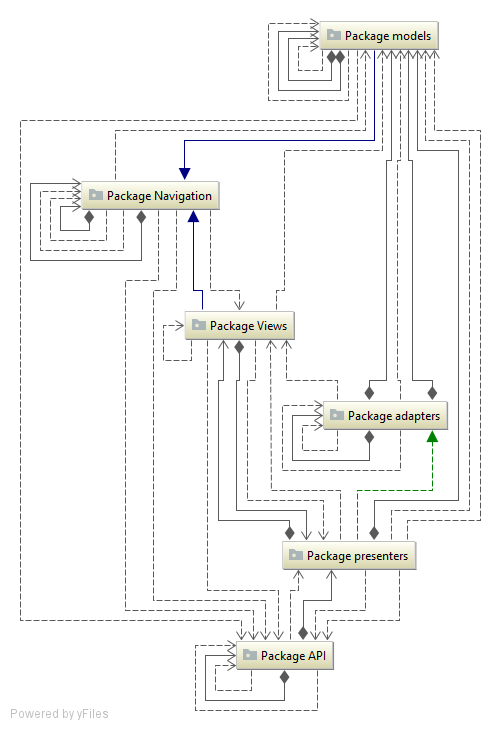
\includegraphics[width=12.5cm,height=6cm,keepaspectratio]{Obrazy/AM_DK_ALL}
			\caption{Schemat ogólny diagramu klas dla Aplikacji Mobilnej}
			\label{Schemat ogólny diagramu klas dla Aplikacji mobilnej}
		\end{figure}
	

		\begin{figure}[ht!]
		\centering
		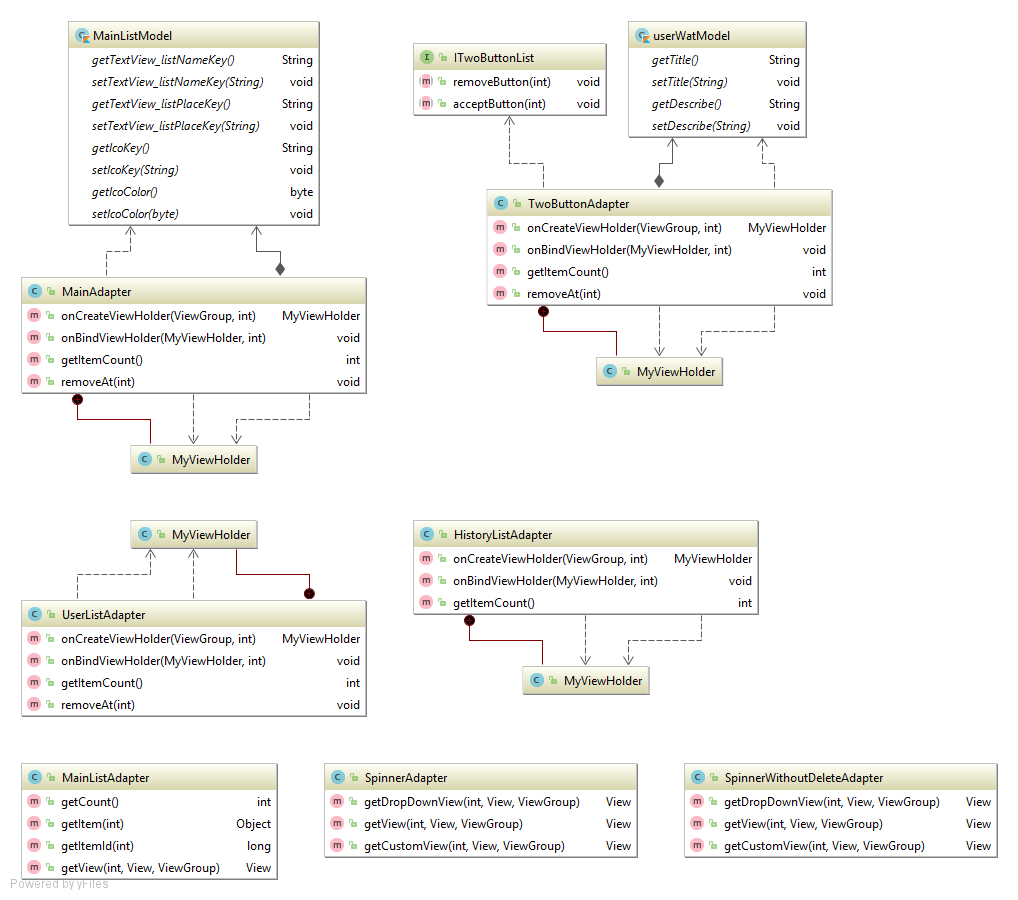
\includegraphics[width=12.5cm,height=10cm,keepaspectratio]{Obrazy/AM_DK_adapter}
		\caption{Diagram klas dla paczki adapters}
		\label{Diagram klas dla paczki adapters}
	\end{figure}
	

	
		\begin{figure}[ht!]
		\centering
		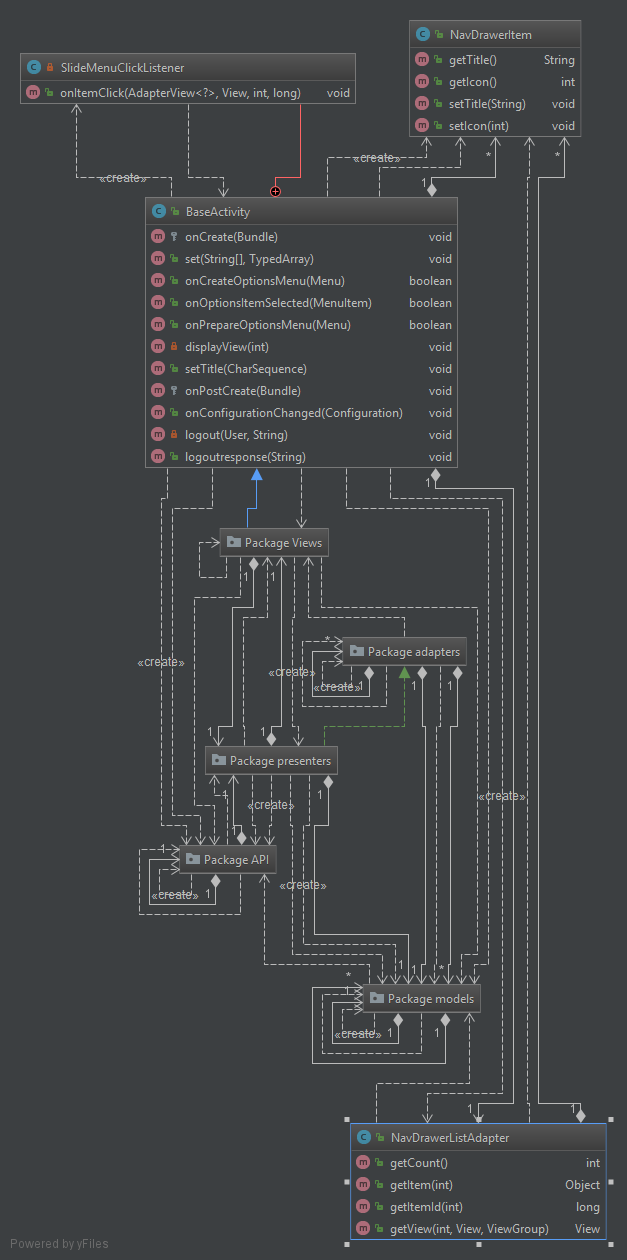
\includegraphics[width=12.5cm,height=10cm,keepaspectratio]{Obrazy/AM_DK_navigation}
		\caption{Diagram klas dla paczki navigations}
		\label{Diagram klas dla paczki navigations}
	\end{figure}

	
	
	
	
	\begin{figure}[ht!]
		\centering
		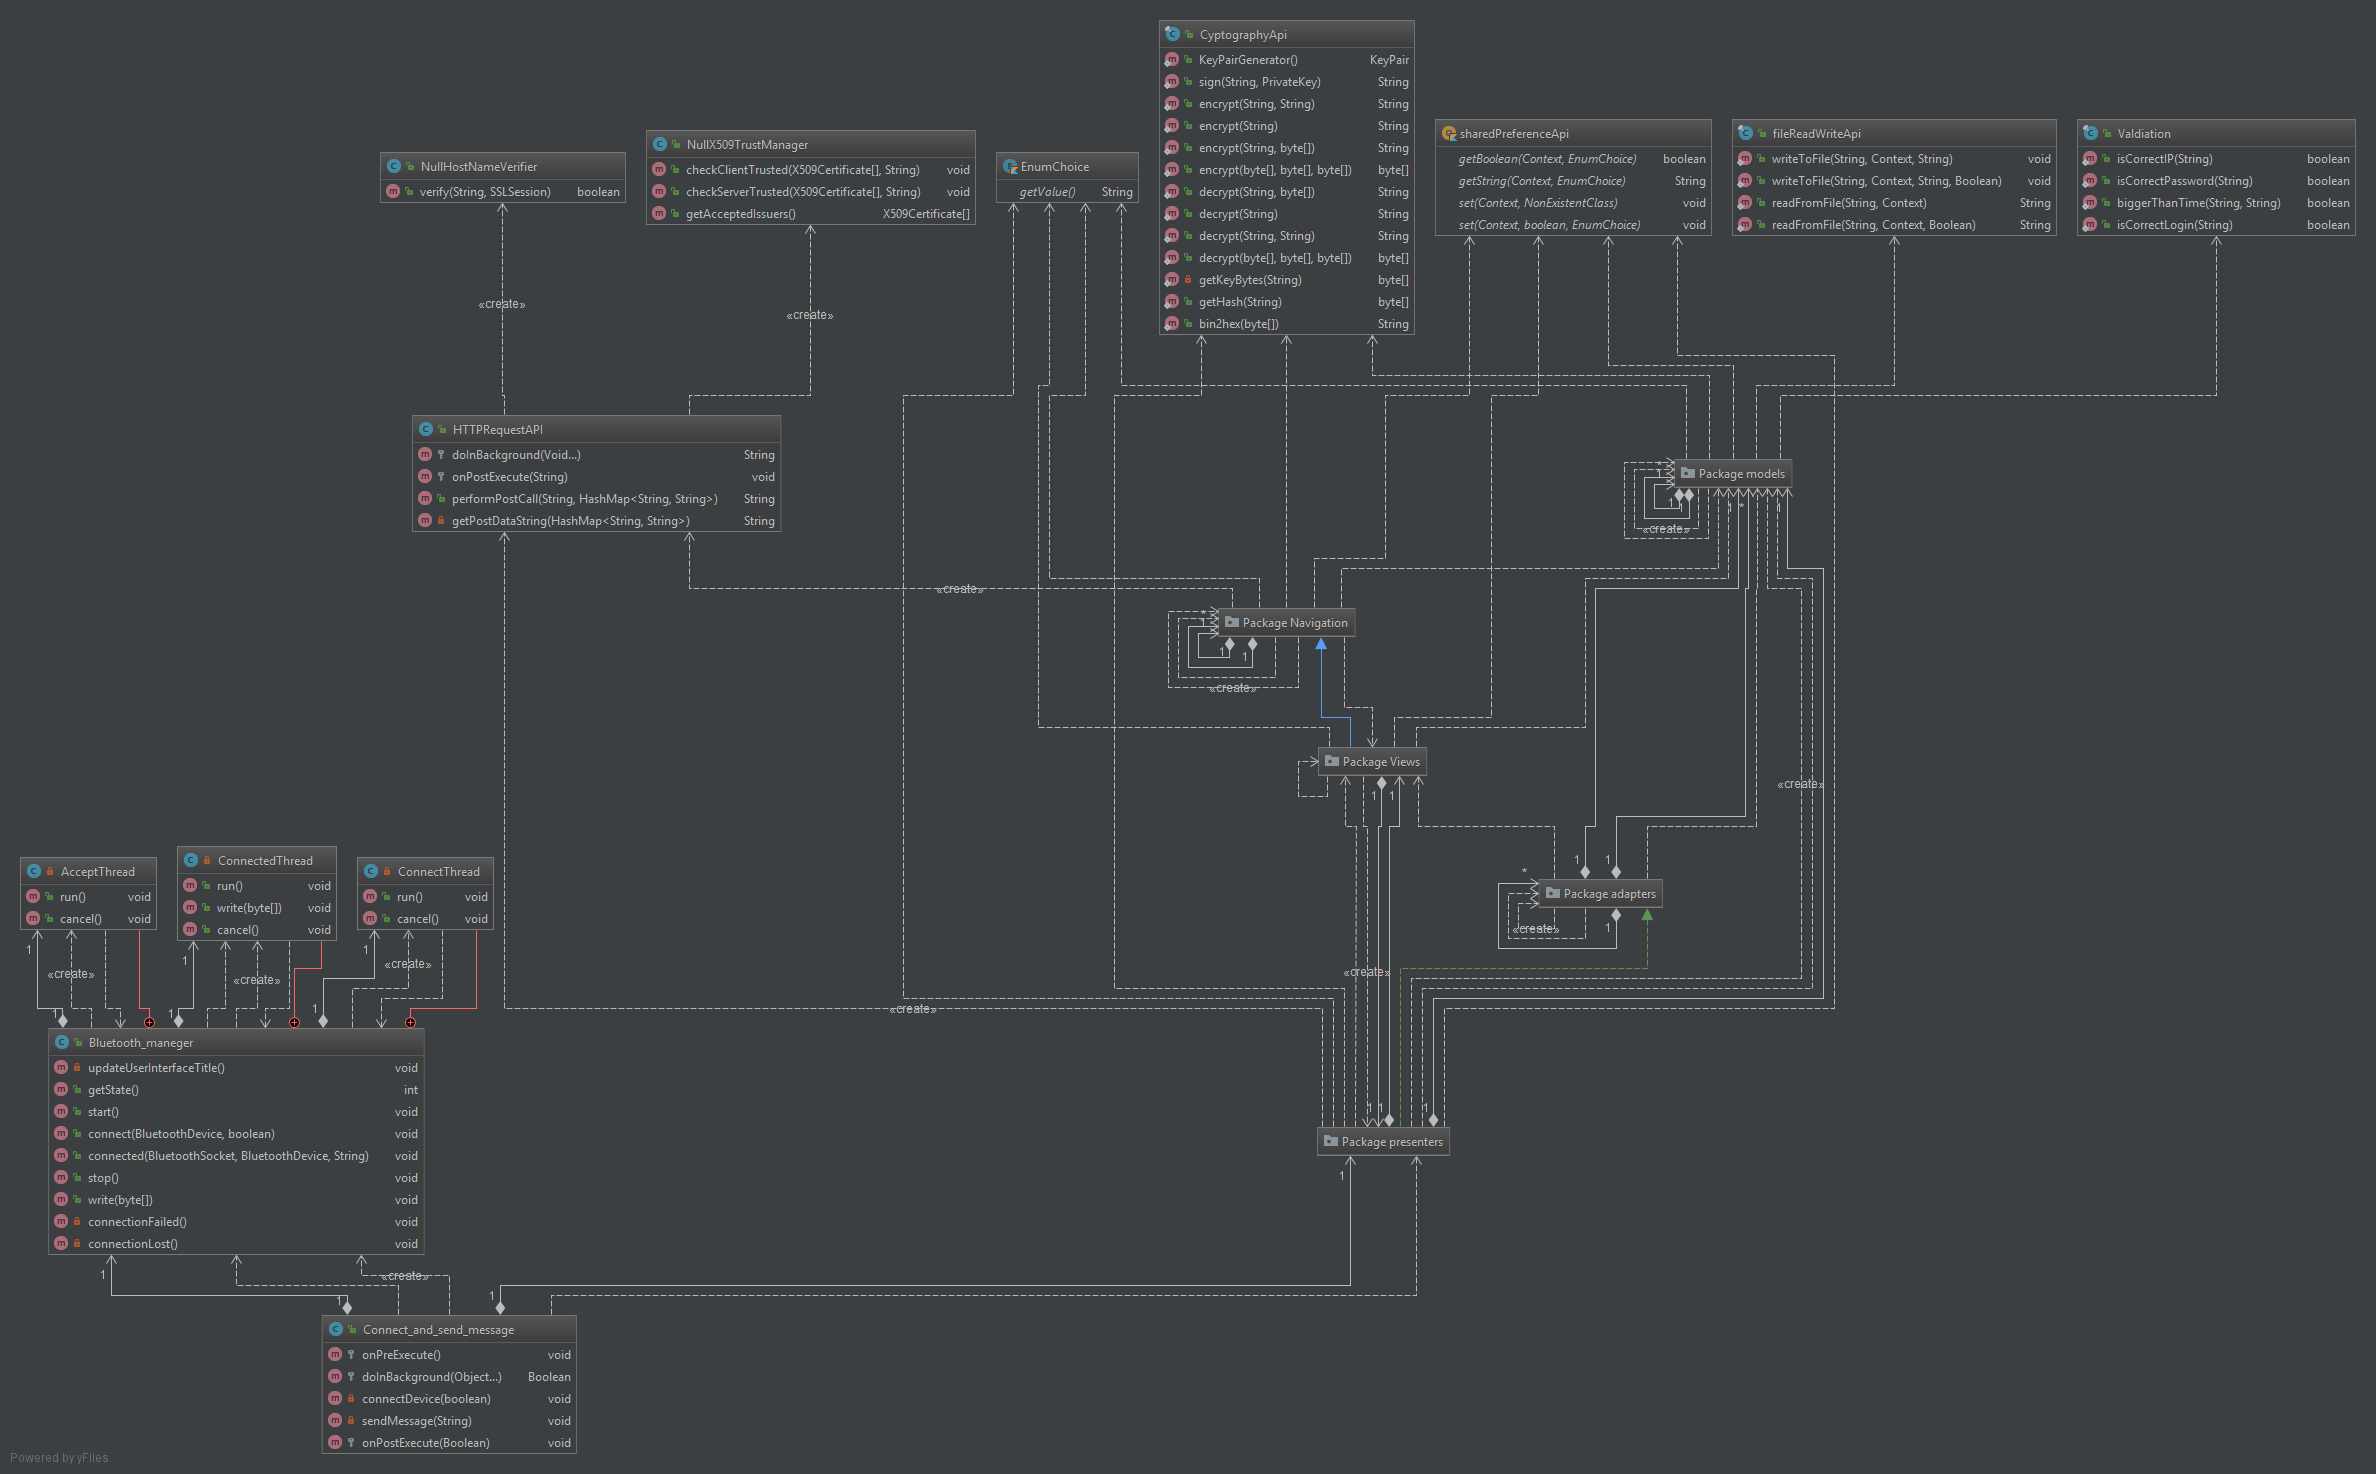
\includegraphics[width=12.5cm,height=16cm,keepaspectratio]{Obrazy/AM_DK_api}
		\caption{Diagram klas dla paczki api}
		\label{Diagram klas dla paczki api}
	\end{figure}

	

	\begin{figure}[ht!]
		\centering
		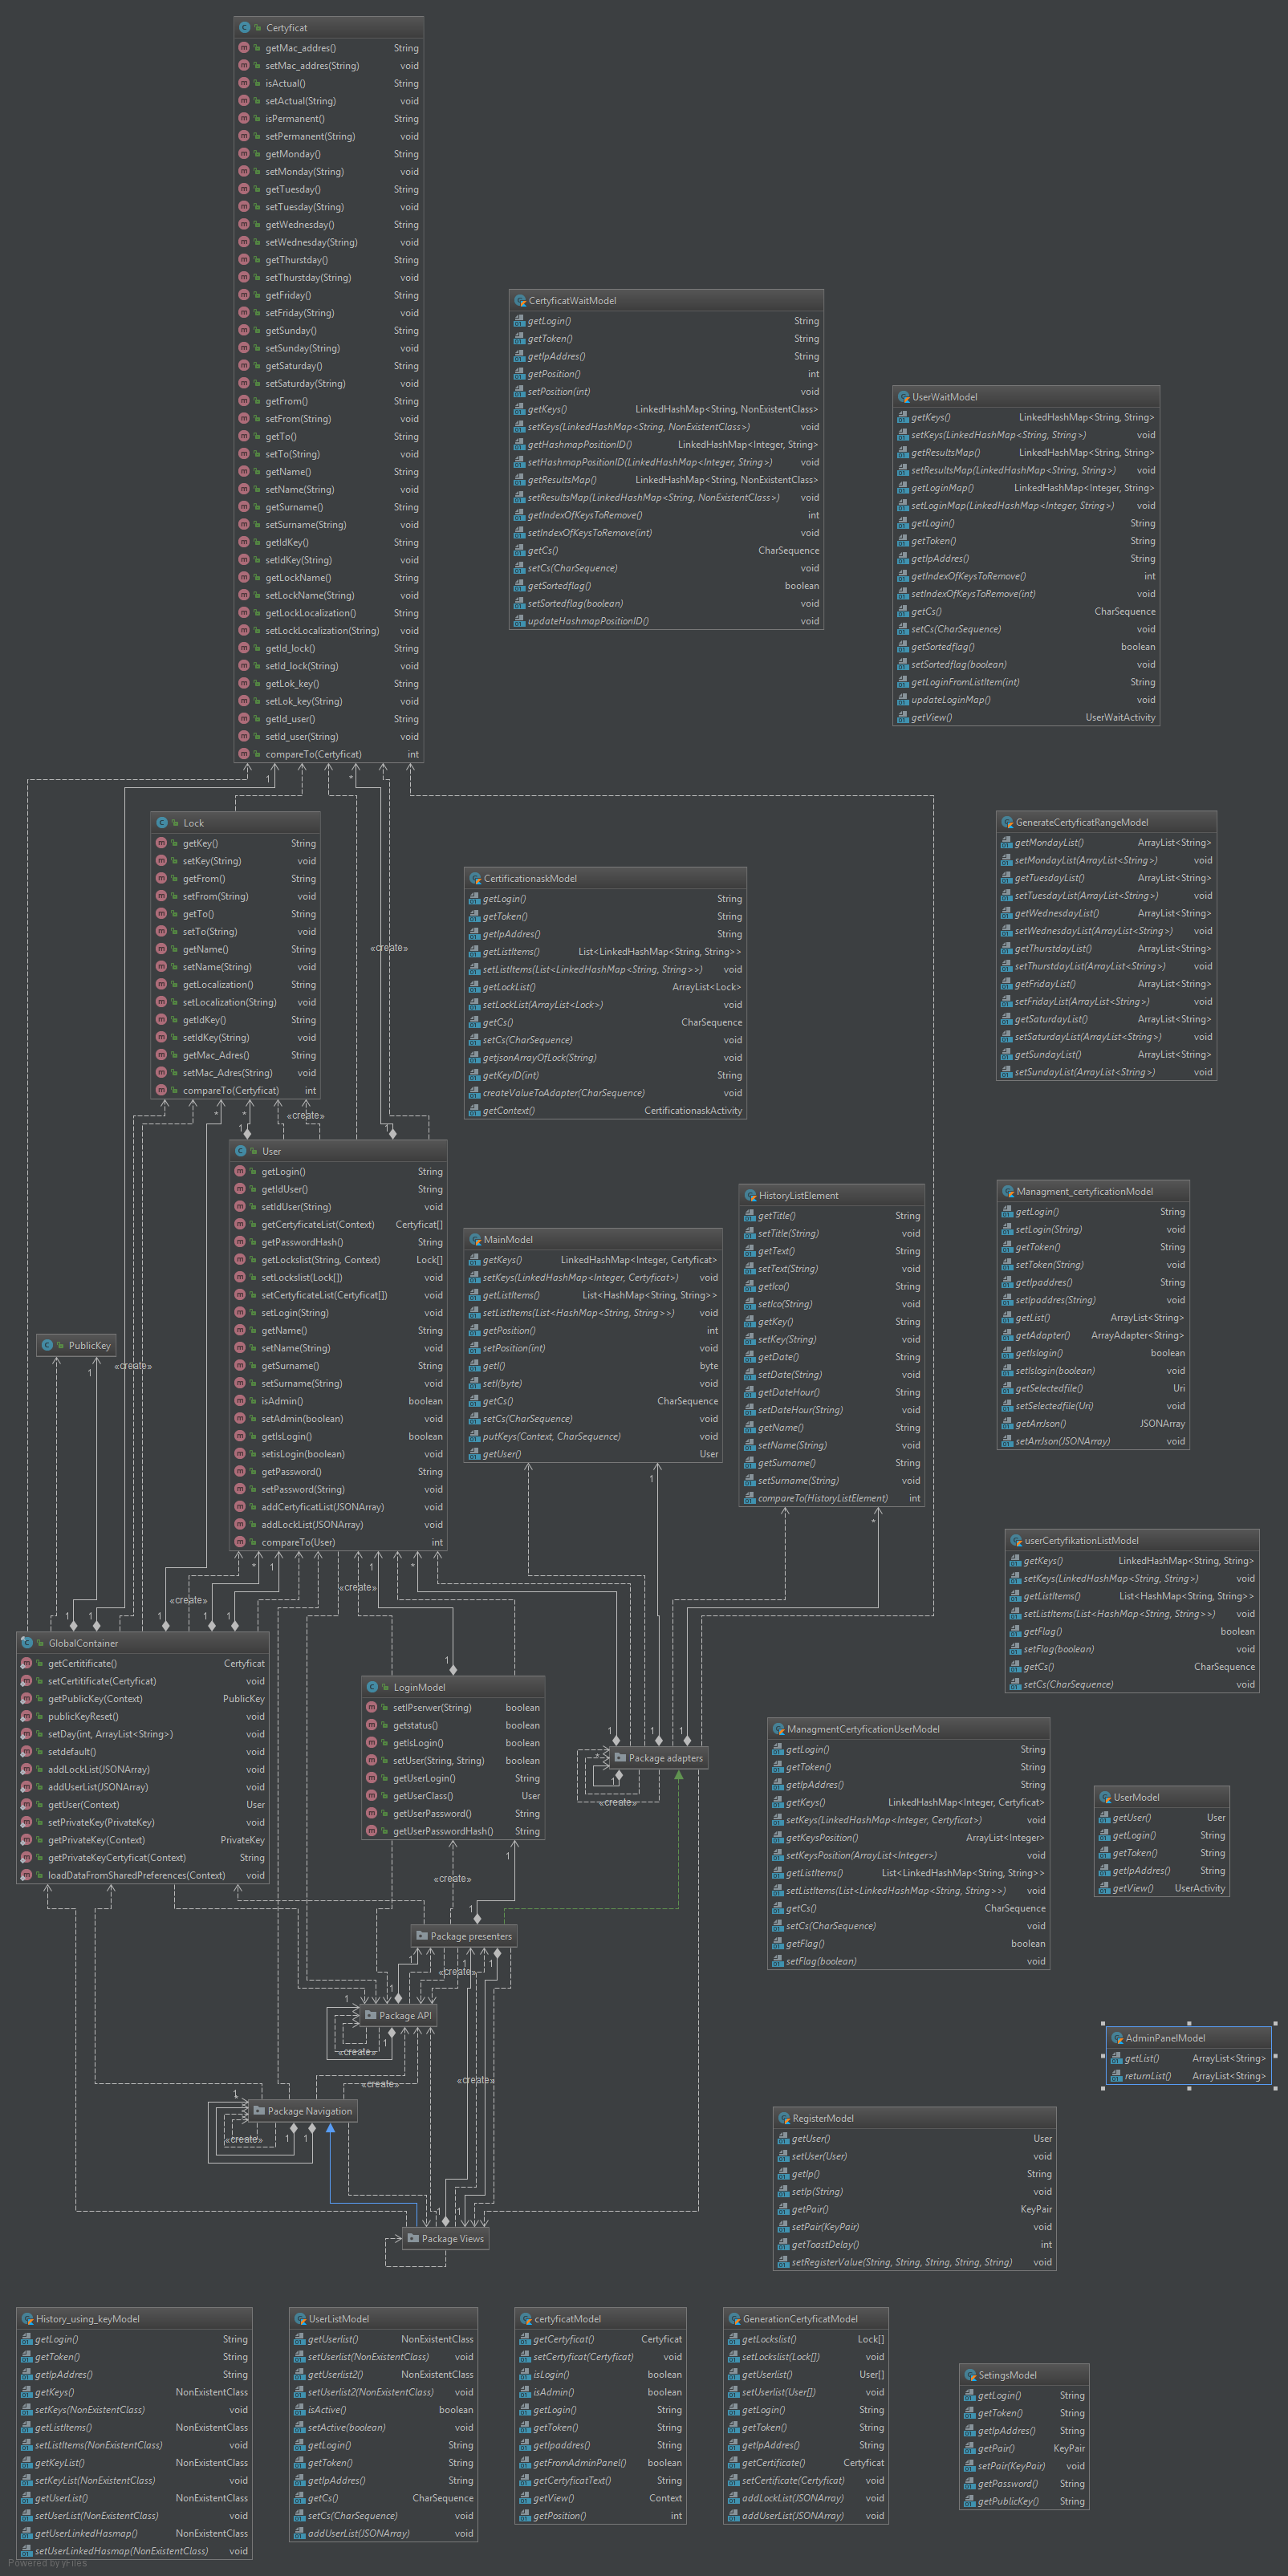
\includegraphics[width=12.5cm,height=18cm,keepaspectratio]{Obrazy/AM_DK_model}
		\caption{Diagram klas dla paczki models}
		\label{Diagram klas dla paczki models}
	\end{figure}

	
\begin{figure}[ht!]
	\centering
	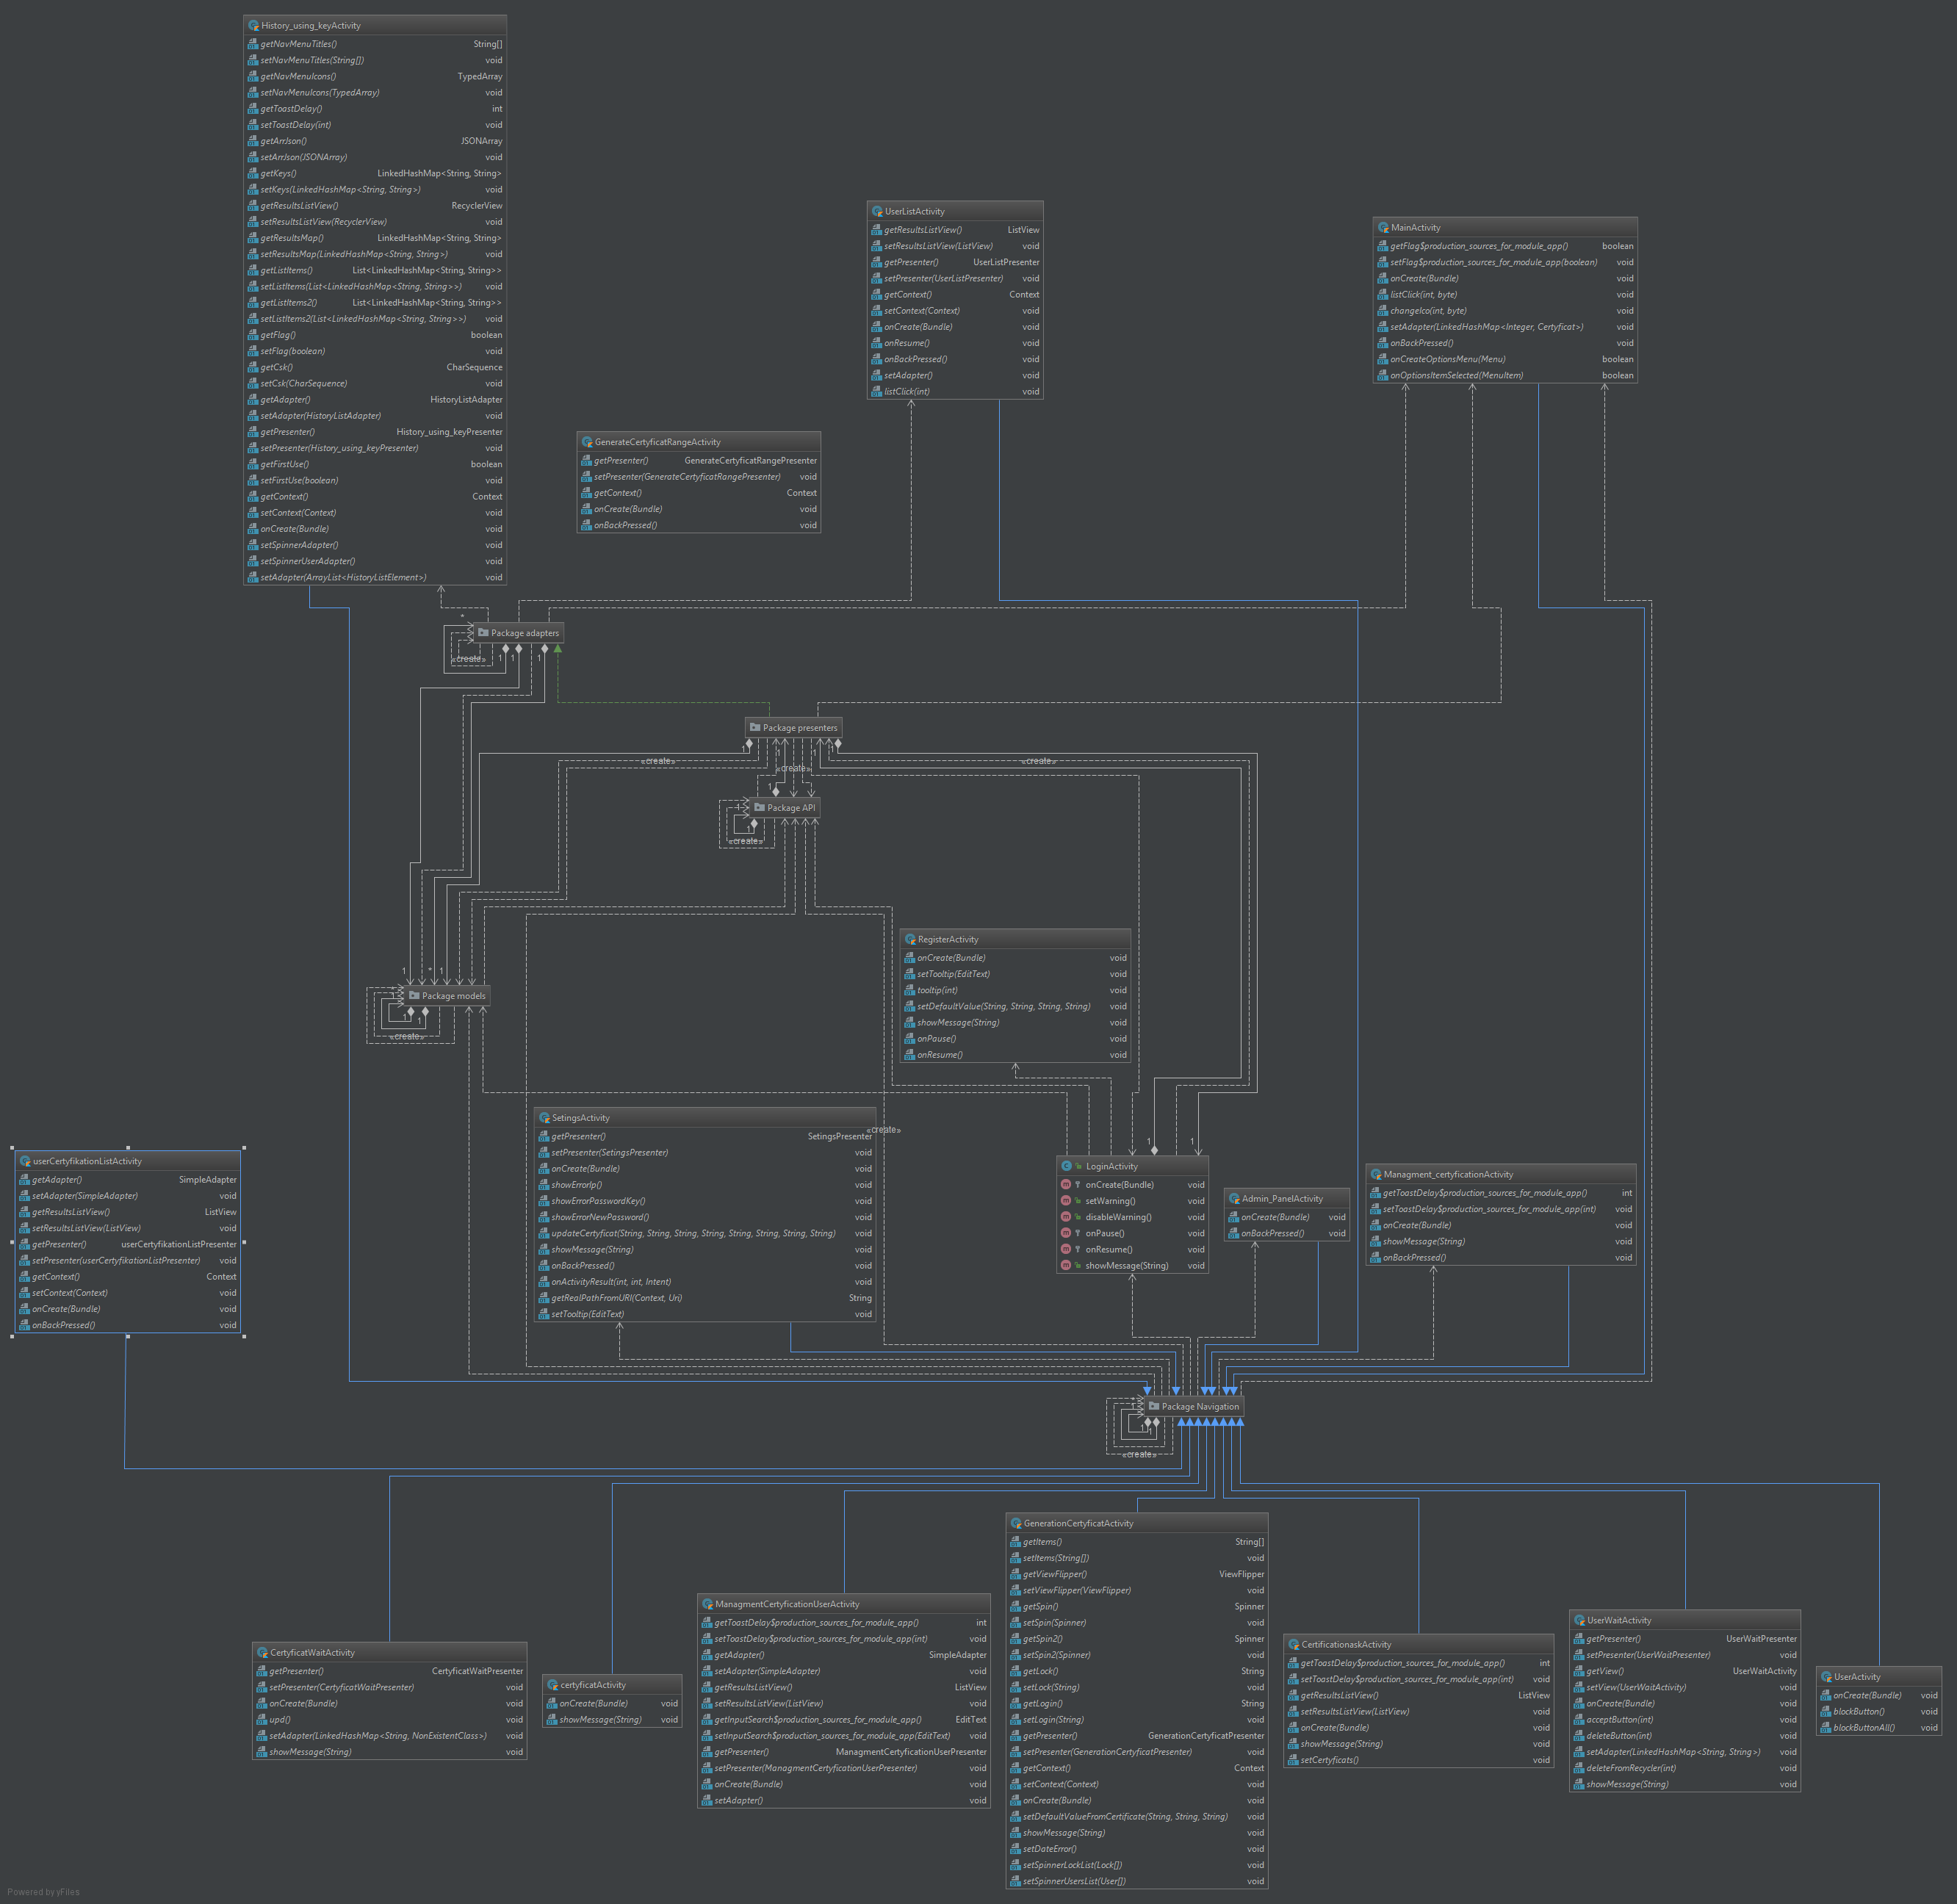
\includegraphics[width=12.5cm,height=12cm,keepaspectratio]{Obrazy/AM_DK_view}
	\caption{Diagram klas dla paczki views}
	\label{Diagram klas dla paczki views}
\end{figure}

		
			Ostatni diagram dotycząćy aplikacji mobilnej przedstawia rozwinięcie paczk Presenter wraz z połączeniami z innymi paczkami
		\begin{figure}[!h]
			\centering
			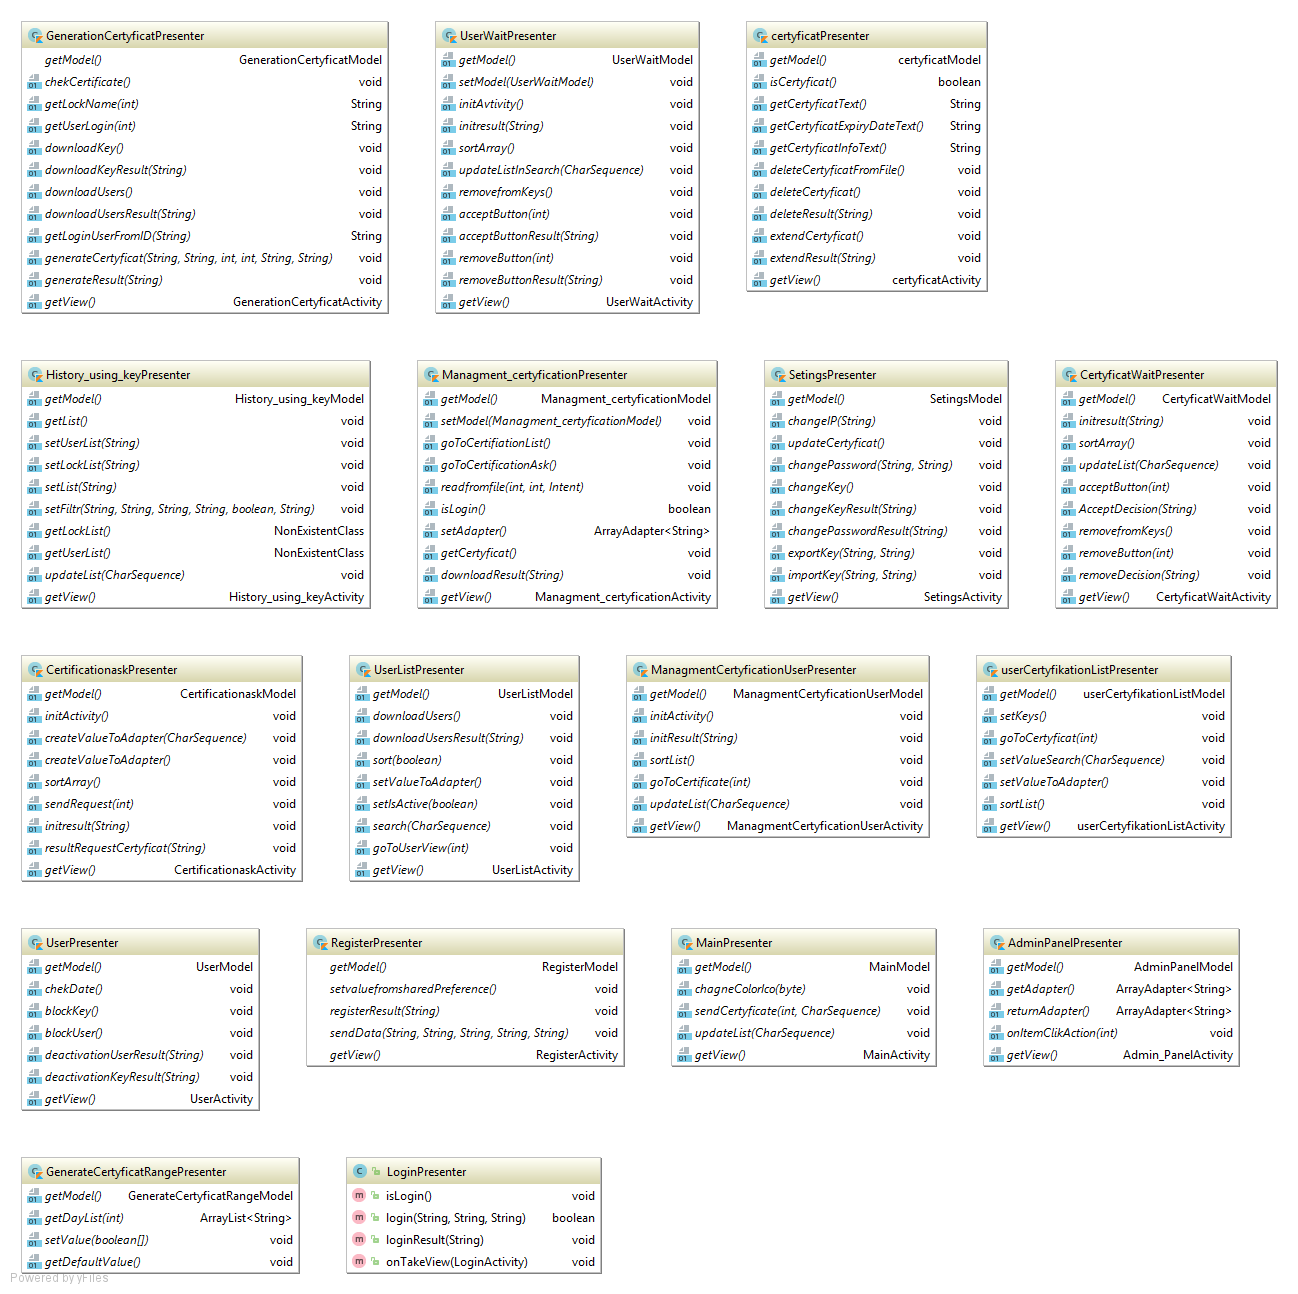
\includegraphics[width=12.5cm,height=14cm,keepaspectratio]{Obrazy/AM_DK_presenter}
			\caption{Diagram klas dla paczki presenters}
			\label{Diagram klas dla paczki presenters}
		\end{figure}
		
		\newpage
		\paragraph{Aplikacja serwera}
		\paragraph{Urządzenie sterujące}
		\paragraph{Moduł zliczania osób}

\newpage		
\subsection{Uproszczony schemat elektryczny systemu}

\newpage
\subsection{Komunikacja modułów systemu z aplikacją  serwera}

	\subsubsection{Komunikaty HTTPRequest pomiędzy aplikacją mobilną, \newline a serwerem}
	\subsubsection{Komunikaty HTTPRequest pomiędzy urządzeniem sterującym, a serwerem}
	
\newpage
\subsection{Protokoły komunikacji pomiędzy urządzeniem \newline sterującym i aplikacją mobilną}

\newpage
\subsection{Interfejs graficzny systemu}

	\subsubsection{Widoki aplikacji mobilnej}
	
	\subsubsection{Widoki strony internetowej systemu}
	
	\subsubsection{Komunikacja człowiek-interfejs}
	
		\paragraph{Komunikaty tekstowe}
		\paragraph{Symbolika ikon}
		\paragraph{Znaczenie kolorystyki}
		
	\subsubsection{Kolorystyka systemu}
	
\newpage
\subsection{Bezpieczeństwo systemu}
	\subsubsection{Projekt infrastruktury klucza publicznego (PKI)}
		\paragraph{Idea PKI}
		\paragraph{Urzedy certyfikujące}
		\paragraph{Klient systemu}
	\subsubsection{Poufność}
	\subsubsection{Dostępność}
	\subsubsection{Integralność}